\begin{figure}[H]
    \centering

    \begin{subfigure}[t]{.6\textwidth}
        \centering
        \begingroup
  \sbox{\tempbox}{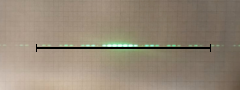
\includegraphics[width=\textwidth,page=1]{figuras/medidas/B4.pdf}}
  \begin{picture}(\wd\tempbox,\ht\tempbox)
    \put(0,0){\usebox{\tempbox}}
    \put(0,0){\includegraphics[width=\textwidth,page=2]{figuras/medidas/B4.pdf}}
    \put(.47\wd\tempbox,.37\ht\tempbox){$4~\Delta y$}
    \put(.48\wd\tempbox,.54\ht\tempbox){$5\Lambda$}
  \end{picture}
\endgroup


        \caption{B4}
        \label{fig:B4}
    \end{subfigure}
    \qquad
    \begin{subfigure}[t]{.6\textwidth}
        \centering
        \begingroup
  \sbox{\tempbox}{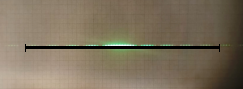
\includegraphics[width=\textwidth,page=1]{figuras/medidas/B5.pdf}}
  \begin{picture}(\wd\tempbox,\ht\tempbox)
    \put(0,0){\usebox{\tempbox}}
    \put(0,0){\includegraphics[width=\textwidth,page=2]{figuras/medidas/B5.pdf}}
    \put(.48\wd\tempbox,.37\ht\tempbox){$5~\Delta y$}
    \put(.46\wd\tempbox,.525\ht\tempbox){$11~\Lambda$}
  \end{picture}
\endgroup


        \caption{B5}
        \label{fig:B5}
    \end{subfigure}
    \qquad
    \begin{subfigure}[t]{.6\textwidth}
        \centering
        \begingroup
  \sbox{\tempbox}{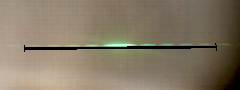
\includegraphics[width=\textwidth,page=1]{figuras/medidas/B6.pdf}}
  \begin{picture}(\wd\tempbox,\ht\tempbox)
    \put(0,0){\usebox{\tempbox}}
    \put(0,0){\includegraphics[width=\textwidth,page=2]{figuras/medidas/B6.pdf}}
    \put(.47\wd\tempbox,.38\ht\tempbox){$5~\Delta y$}
    \put(.595\wd\tempbox,.54\ht\tempbox){$6\Lambda$}
  \end{picture}
\endgroup


        \caption{B6}
        \label{fig:B6}
    \end{subfigure}

    \caption{Fotos dos padrões de difração das fendas B}
    \label{fig:B}
\end{figure}